% !TEX program = xelatex
\documentclass[letterpaper,12pt]{article}
\usepackage{tabularx} % extra features for tabular environment
\usepackage{amsmath, amssymb, mathtools}  % improve math presentation
\usepackage{graphicx} % takes care of graphics including machinery
\usepackage{setspace}
\usepackage{url}
\usepackage{chemfig}
\usepackage[version=4]{mhchem}
\usepackage{seqsplit}
\usepackage[margin=2.54cm,letterpaper]{geometry} % decreases margins
\usepackage{caption}
\usepackage{adjustbox}
\usepackage{booktabs}
\usepackage{cite} % takes care of citations
\usepackage[final]{hyperref} % adds hyperlinks inside the generated pdf file
\hypersetup{
	colorlinks=true,       % false: boxed links; true: colored links
	linkcolor=blue,        % color of internal links
	citecolor=blue,        % color of links to bibliography
	filecolor=magenta,     % color of file links
	urlcolor=blue         
}
\usepackage{blindtext}
\usepackage{amsfonts}
\usepackage{tikz}
\usepackage{standalone}
\usepackage{xcolor}
\usepackage{bookmark}
\usepackage{chemformula}
\usepackage[para]{footmisc}
\usepackage{subcaption}

\setchemfig{atom sep=4em}
\captionsetup{justification=centering, font=small}
\definecolor{darkgray}{gray}{0.3}
\newcommand{\annot}[1]{\textcolor{darkgray}{\textit{#1}}}

\renewcommand{\footnoterule}{%
  \kern-3pt % space above the rule
  \hrule width \textwidth height 0.4pt
  \kern5pt % space below the rule
}

\usepackage{fontspec}
\setmainfont{Arial} % replace 'Arial' with your preferred 

\begin{document}
% TODO: Make the title page centered and in a single page
\title{\vspace{-2em}Extraction of Ortho-Vanillin via Steam Distillation}
% \vspace{-0.5cm}
% \author{Harsh Agrawal (CID - 02320622) \\ Department of Bioengineering, Imperial College London}
\date{}
\maketitle
\vspace{-2em}

\begin{spacing}{1.5}
    \noindent \textbf{Name}: Harsh Agrawal\\
    \textbf{CID}: 02320622 \\
    \textbf{Yield}: 0.325 grams \\
    \textbf{R$_f$}: 0.317 (Ortho-vanillin) and 0.167 (Vanillin) \\
\end{spacing}

\section*{Questions}
\subsubsection*{1. Assume that you didn't know ahead of time whether the ortho-vanillin or the vanillin would distil over to the second flask. How could you determine the identity of the distilled compound? Outline three possible tests that could be performed}

\begin{enumerate}
    \item \textbf{Melting Point Test}: Due to the difference in the melting points of vanillin and ortho-vanillin, the melting point test can be performed. The obtained distillate can be crystallized, and a few grams of the solid product can be loaded into a capillary tube and gradually heated inside the melting point apparatus to observe the temperature at which the crystals liquefy. If the temperature recorded is in the range of 40$^{\circ}$- 42$^{\circ}$ C, then the obtained is Ortho-Vanillin. If the temperature recorded is in the range of 81$^{\circ}$- 83$^{\circ}$ C, then the obtained is Vanillin.
    \item \textbf{H-NMR}: H-NMR can also be performed to identify vanillin from ortho-vanillin. The differential placement of the aldehyde group in vanillin and ortho-vanillin will produce different splitting patterns that can be analyzed to determine the identity of the compound.
    \item \textbf{Thin Layer Chromatography}: Due to the difference in relative polarity of vanillin and ortho-vanillin, thin-layer chromatography can be performed. The obtained distillate can be dissolved in a suitable solvent and spotted on a TLC plate. If the obtained R$_f$ value is near 0.1 to 0.15, then the substance is vanillin. Contrarily, if the obtained R$_f$ value is in the range of 0.3 to 0.35, then the obtained substance is ortho-vanillin.

\end{enumerate}

\subsubsection*{2. If the compound of interest had to be distilled under reduced pressure, what modification could you make to the apparatus to do so?
}

To carry our reduced-pressure distillation, a vacuum pump can be attached to the distillation apparatus. The choice of the vacuum pump can be made according to the pressure reduction. Oil-sealed vacuum pumps can offer higher vacuum levels, while dry pumps such as scroll pumps are preferred to prevent contamination of the distillate. The pump is usually connected near the condenser.

\subsubsection*{3. What difficulties might occur if there was no way to cool the condenser?
}
There are several difficulties that might occur if there was no way to cool the condenser.
\begin{itemize}
    \item \textbf{Inadequate condensation of distillate}: If the condensor is not cooled, the distillate wouldn't condense to a liquid state and thus would not travel to the recieveing flask.
    \item \textbf{Loss of distillate / Reduced Yeild}: Due to this, the amount of collected distillate would be reduced, leading to a lower yield of the desired compound.
    \item \textbf{Safety Hazard}: The lack of cooling might lead to a gaseous buildup in the distillation apparatus, which could pose safety hazards such as leakage of potentially toxic gaseous products, over-pressurization and breaked of the apparatus, and over-heating of the appartus.
\end{itemize}

\subsubsection*{4. What simple technique requiring minimal equipment could be used to determine whether the distillation had succeeded (i.e. whether the distilled liquid contained one component or two)?
}
A simple technique that can be used to assess whether the distillation was successful is to measure the boiling point of the collected distillate.

This requires very minimal equipment --- a hotplate, and a thermometer. The boiling point of the collected distillate can be measured by heating the distillate in a round-bottom flask and observing the temperature at which the distillate starts to boil. If the temperature at which the distillate starts to boil matches the boiling point of the more volatile compound (ortho-vanillin in our case), then we can conclude the obtained distillate is pure. Whereas if the boiling point of the distiallate is lower than the boiling point of the more volatile compound, then it can be concluded that the distillate still contains both the compounds.

\subsubsection*{5. Describe another technique you could use to separate vanillin and ortho-vanillin. Draw a diagram of the apparatus and explain briefly what the main parts do.
}
\begin{figure}[!ht]
    \centering
    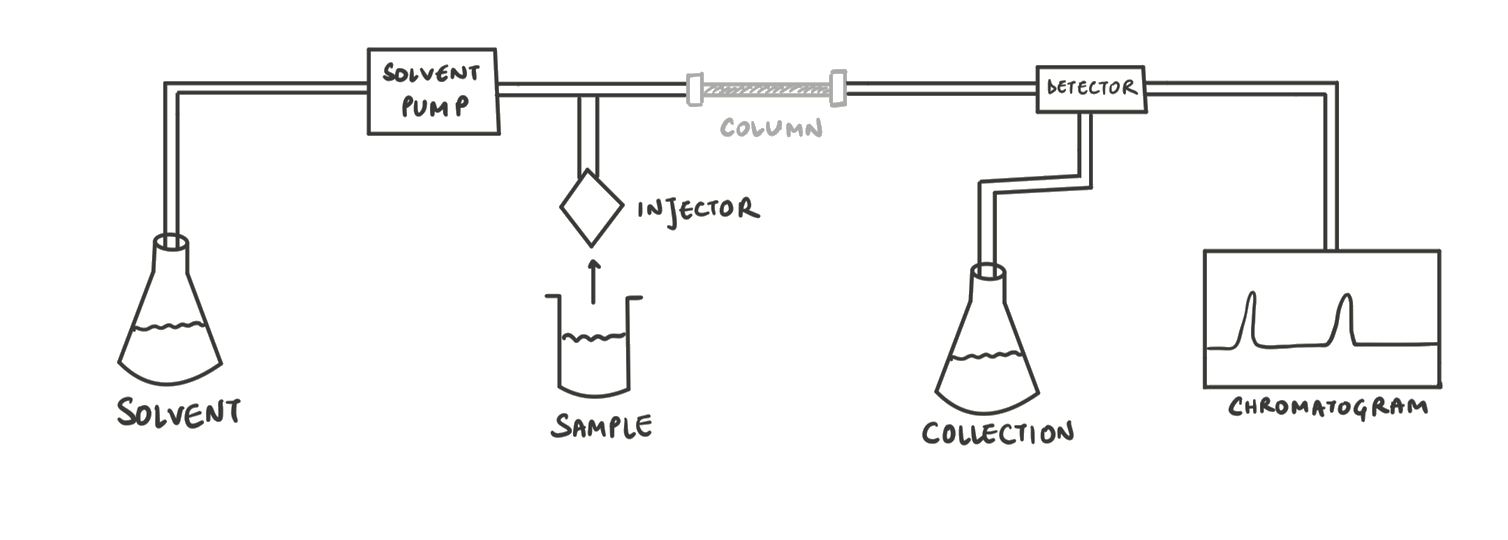
\includegraphics[width=1\textwidth]{figures/hplc.png}
    \caption{Simple HPLC Apparatus Setup}
\end{figure}
High Performance Liquid Chromatography can be used to effectively seperate vanillin and ortho-vanillin. Reversed-Phase HPLC is more typically used. The apparatus consists of:
\begin{itemize}
    \item \textbf{Pump}: Used to push the mobile phase through the column at a constant flow rate.
    \item \textbf{Injector}: Used to inject the sample into the column.
    \item \textbf{Column}: Consists of a narrow tube packed with a stationary phase. The sample is separated based on the differential interaction of the compounds with the stationary phase and the mobile phase.
    \item \textbf{Mobile Phase}: In a reversed-phased HPLC, the mobile phase consists of a polar solvent mixture, often water combined with a polar organic solvent.
    \item \textbf{Stationary Phase}: The stationary phase in reversed-phase HPLC is usually a non-polar material, that interacts more strongly with less polar analytes in the sample.
    \item \textbf{Detector}: The detector is used to detect the eluted compounds. The detector can be a UV-Vis detector, a fluorescence detector, a refractive index detector, an electrochemical detector, among others. The choice is made on the type of the compound being analyzed.
\end{itemize}
The pump is used to push the mobile phase through the column, which already contains a stationary phase. The sample is also injected into the column using the injector. Due to the differential interaction of Vanillin and ortho-vanillin with both the phases, they will pass the columns at different times.

In reversed-phase HPLC, retention is dominated by the hydrophobic/non-polar interactions between the analytes and the stationary phase. This is why the more polar compound will elute first followed by the less polar compound. The detector can used to detect the eluted compounds. To seperate vanillin and ortho-vanillin, a seperate collection apparatus can be connected to the detector through which both the samples can be collected at the end in different collection tubes.

The solvent can then be evaporated to obtain the pure compounds. As specified earlier, the boiling point test can be performed to assess the purity of the seperated compounds.

\end{document}
